\section{Delft-FEWS flow forecasting system}
\acrshort{fews} is developed by Deltares in the Nethaland with targeted for use by operational forecasting agencies. %The software is freely available to download and setup. Tutorials and User setup guide \cite{DeltaresPublicWikiDelft-FEWSGuide} are available with well documentations. For non-commercial users need to have the licence agreement to use the system. And get new system updates. However, investments in new developments in the system are normally paid for by its users. 
The code base of \acrshort{fews} is currently not fully open source. %But configuration guides and generic adapter module integration code examples are available for the users.
Most if the models are using model-centric approach such as inputs need to be in the format of specific to the model. Also, the outputs produced by the model are specific to the model and hard to utilize by another systems (e.g., FLO2D). As \acrshort{fews} %is using much more 
uses a modular approach it is easier to integrate new models.% into the \acrshort{fews} system. 
Thus, \acrshort{fews} can be consider as an integration framework or a middleware for the models.
\dbc{Cite Fews. Provide only the key details. It's sufficient say whether its commercial or open source. Do this for all other solutions discussed. Middleware is a single word. Check other places.}

Forecasting processes are constructed as a combination of modelling steps and data transformation algorithms. These are then combined to provide required forecast capabilities. Flexibility is achieved through integrating new models and algorithms into the code base \cite{Werner2013TheSystem}. Delft-FEWS system contains no inherent hydrological modelling capabilities within its code base. Rather it is a framework which can use to integrate into the system and create work flows for forecasting.

Are proposed by Haggett \cite{Haggett1998AnWales} key elements of a forecasting system include detection, forecasting, dissemination and warning, and response. Within these four steps, \acrshort{fews} focuses on the forecasting step. The primary objective of this step is to provide additional lead time through predictions of short term future hydro-meteorological conditions \cite{Werner2005FloodCatchments}. It is true that, with providing accurate predictions with greater lead time can reduce the level of destruction. In order to do the forecasting, the system should be capable of integrating real-time data from hydrological and meteorological observation networks, and the dissemination of prediction results through appropriate products to the warning process.

In figure \ref{fi:fews_schematic} show a schematic view of the connection between the forecasting system to real time data acquisition systems and dissemination systems. The widely using concept is using meteorological forecast data to get precipitation and, then using hydrological and hydraulic model chain to predict the level affect on the ground. The hydrological and hydraulic model should be design based on the ground. Basically ground should be analyze geographically and divide into the catchments. Based on the affected catchment, it can be further divide into sub areas in order to reduce the complexity of the simulation task. Ideally the forecasting system should therefore be flexible to allow change to models and data, while keeping the way forecasters work with it as constant as possible.
 
\begin{figure}[htp]
    \centering
    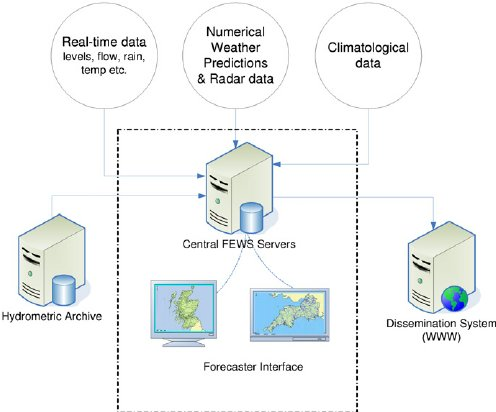
\includegraphics[width=0.7\textwidth]{fews/Schematic-structure-of-a-fl-ood-forecasting-system-showing-the-position-of-Delft-FEWS_W640.jpg}
    \caption{Schematic structure of a flood forecasting system including \acrshort{fews} and links to other primary systems within the operational environment \cite{Werner2013TheSystem}.}
    \label{fi:fews_schematic}
\end{figure}
\dbc{Most figures are of low quality. You need to make sure figure resolution/quality is not lost. Dot should come after reference no. Fix all places.}

The foundation of \acrshort{fews} is data-centric, with a common data-model through which all components interact. All time series data (both scalar and gridded) are stored in this common data-model in a database. Modeling capabilities are then linked to the system through one of the interfaces provided to the data-model \cite{Werner2013TheSystem}. As mention in the paper, having a common data-model make easy to store data in an efficient way. Operations like reporting and sharing the data also make it easy for integrate models. But the problem with this approach is, handling the multiple data formats. \acrshort{fews} overcome this issue with introducing adapters for most of commonly used data formats. This is a good feature which enable users to easily import data into the system. But at the same time, it's adding additional complexity into the system.

Time series data is additionally either scalar, vector, or gridded data, though all different types are uniformly stored as binary objects in a time series table. None of the functional components (including the linked models) have direct access to the times series table, which is accessible only through the data access module \cite{Werner2013TheSystem}. As it explained in the system interpretation, every time all the data access need to go through the data access module which causing to adding more cost in data access. Since it is storing the different data types as binary objects, there is a penalty in converting data into binary objects and vice a versa. Storing all the data in a time series table causing all the request come into a single data point. Even it gives the advantage of accessing all the data at one place. Since screaming big amount of data is causing a heavy load on the system, causing to slow down the performance on trying to use the system on large set of data.

Given above drawback on storing the data in the system, within the \acrshort{fews} data model, time series are uniquely identified by their location and data type, as well as an id related to the source of the data (e.g. the external source or hydrological model of which the time series are a result) \cite{Werner2013TheSystem}. This gives an opportunity to index the data base on above key fields and store the data separately, in order to take the advantage of putting multiple data resources into the system. As an example, instead of storing the data at a single timeseries table, it is possible to separate and index the database based on source such as external source or hydrological model of which the time series are a result. Or separate by data type and store in multiple storage give the capability for the system to scale with factor of identical types that can be identified. Example of separation by data types of scalar, vector and gridded will increase the scaling factor by 3x.

Data processing and manipulation is a required process in weather forecasting. Most of the data that is imported from external sources is not at the appropriate temporal and spatial scale to be applied as an input to a forecasting model, or to be used directly in product generation. As a consequence, generic data processing steps form the predominant effort in most applications of models in the forecast environment. Some examples include data validation, serial and spatial interpolation, aggregation and dis-aggregation, and merging data \cite{Werner2013TheSystem}. This a vital feature in a forecasting system, and affect on the quality and accuracy of the predicted data outputs. Because of the common data model concept in the \acrshort{fews}, data processing via these function is much effective. The system is self provided some of the generic functions for data processing, but for more complex algorithms can be developed as a new Java class coded to communicate with the application programming interface (API). It obvious that for additional feature integration, user should implement the new functional extensions via Java programming language. Users does not have the flexibility of develop with some other languages they are familiar with or use the support from another language. As an example, Python language is easy to use for beginners and many of data scientists are using this programming language for development and it has many data available libraries for data processing. But in the \acrshort{fews} users do not ave the capability to take the advantage of such existing things.

\begin{figure}[htp]
    \centering
    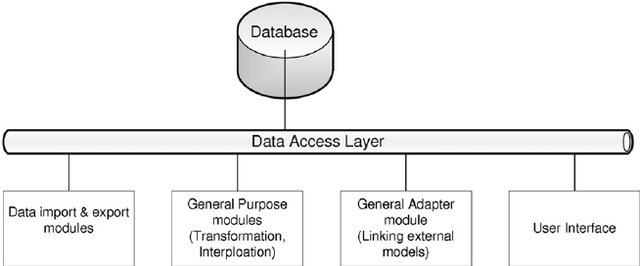
\includegraphics[width=1.0\textwidth]{fews/Architecture-of-Delft-FEWS-showing-the-data-base-the-data-access-layers-and-examples-of_W640.jpg}\\
    \caption{Architecture of \acrshort{fews} % showing the data base, the data access layers and examples of functional modules that communicate through the data access layer. 
    \cite{Werner2013TheSystem} }
    \label{fi:fews_data_layer}
\end{figure}
Most of the library of functions provided work equally on scalar and gridded time series. As with all other modules this communicates with the database solely through the data access layer as shown in \ref{fi:fews_data_layer} \cite{Werner2013TheSystem}. As it shown in the figure, it is clearly showing that, the system is depends on single database and via the data access layer all the requests are coming to the database though a connection. It is possible to setup and connect to a enterprise level database with clustering and shading as a paid solution, in order to serve many requests as possible. But the design it self inherently suffer with the database bottleneck which effected on running a large set of timeseries or models.

\begin{figure}[htp]
    \centering
    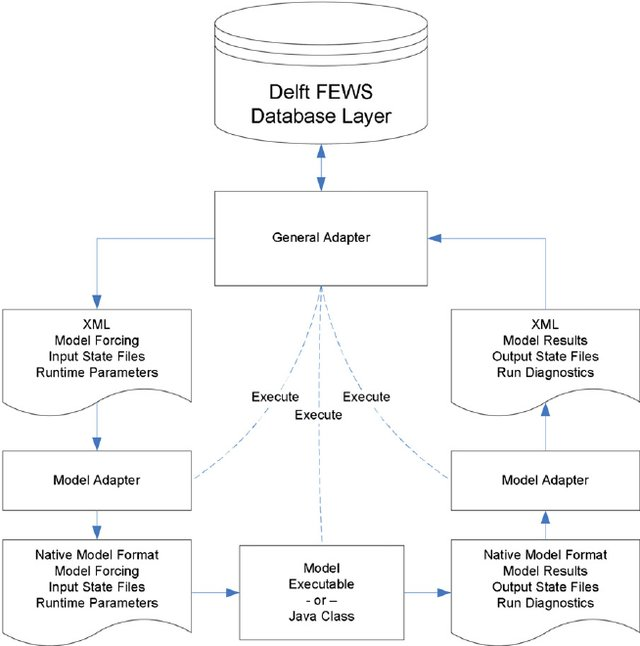
\includegraphics[width=0.8\textwidth]{fews/Linking-Delft-FEWS-with-external-models-The-fi-gure-shows-the-fl-ow-of-data-through-XML_W640.jpg}\\
    \caption{ Linking \acrshort{fews} with external models. The figure shows the flow of data through XML and native model formats using solid lines, while executable commands are shown by dashed lines. \cite{Werner2013TheSystem} }
    \label{fi:fews_general_adapter}
\end{figure}
On of the simple and most effective feature in the \acrshort{fews} is open approach to integration of models and data. This approaches the concept of the open modeling framework proposed by \cite{Kokkonen2003InterfacingXML}. It simply gives the flexibility to allow operators to integrate more models as well as variations of the same model and come up with new integration flows as much as possible.
\acrshort{fews} generates the input data as a set of XML files to a defined location; an adapter developed specifically for the model in question transforms this to the required native format in a pre-processing step; \acrshort{fews} executes the model; and the adapter to that model then converts the native formatted results into XML formatted files in a post processing step. \acrshort{fews} subsequently imports the results into the database from the XML files (see Fig. \ref{fi:fews_general_adapter}) \cite{Werner2013TheSystem}. The process is simple and consistence through out all the model integration. The model execution is done by the \acrshort{fews} or the model adapter which is causing tide coupling into the execution process in the system. Users does not have the flexibility to run the models with different configurations such as running with parallel execution. That may be overcome by triggering a external process at the execution time, but it introducing more difficulty for handling after model executed successfully, preceding to the next step in the process. This part of the system feature is not focus on the \acrshort{wdias} and user has to come up with own flow or use existing scientific flow management system. But it is a concept that need to be discuss and understand properly in order to design a data integration and assimilation system.

Exchanging data with the model is primarily through XML files. In some cases these XML files may become very large, which may lead to I/O bottlenecks and subsequent performance issues \cite{Werner2013TheSystem}. This issue is thoroughly discussed previous paragraphs and the authors of the \cite{Werner2013TheSystem} seems to be notice and accept it here. For overcome this issue they introduced the file-based exchange of data. This includes the use of binary-XML files, streaming files through memory, and the use of \acrshort{netCDF} files. But far as for users it seems to be adding more complexity and context in order to get higher performance via the system.

If particular adapter for a model is not present in the list of \acrshort{fews} adapter, user has the flexibility to implement an adapter for it. The effort of developing an adapter for a model code not previously integrated with \acrshort{fews} will vary depending on the complexity of the model I/O formats \cite{Werner2013TheSystem}. If user wants to use existing adapter and need to configure something not supported via the existing adapter, it is hard to get done. Also there are some cases it is hard to develop an adapter or running alongside with the \acrshort{fews}. As an example FLO2D model is using for hydrologic modeling and the model is only support only on Windows based operating systems. If you setup the system on Linux base operating system and using Linux based models, it is hard for users to come up with a solution for integrating the FLO2D models.
The final step and one of important feature is exporting the data from the system in useful manner. %\acrshort{fews} supports three main forms of product generation, namely:
%\begin{itemize}
%\item Generate web reports with graphs, tables as well as summary reports
%\item Export time series in a variety of formats
%\item External applications actively retrieve data from the system
%\end{itemize}
The forecasting process is often a sequence of steps, starting with the import of data, a number of data processing and modeling steps, and culminating in the generation of products to be disseminated to the warning process. This is supported via the work flow process in the \acrshort{fews}. The scope of the \acrshort{wdias} is not focus on adding such a feature in the system, rather user have to use scientific work flow management system or come up with own version of work flow.

When running sequential steps within a work flow in \acrshort{fews}, each step is run for the full time window required (e.g. the lead time of the forecast) before moving on to the next step. This precludes tightly coupling of models, even explicitly \cite{Werner2013TheSystem}. As it mentioned above, users can run multiple models parallel or run those sequentially as needed. 
\dbc{It's "e.g.,". Fix all places. }